\section{Exercise 3}
Cho sơ đồ mạch điện sau, vẽ lại mạch sao cho mạch thể hiện rõ sự nối tiếp và/hoặc song song giữa các điện trở. Sau đó tính điện trở tương đương giữa A và F, điện thế tại A, B, C, D và E. Cuối cùng, sử dụng mô phỏng để kiểm tra phép tính.
\begin{figure}[!htbp]
    \centering
    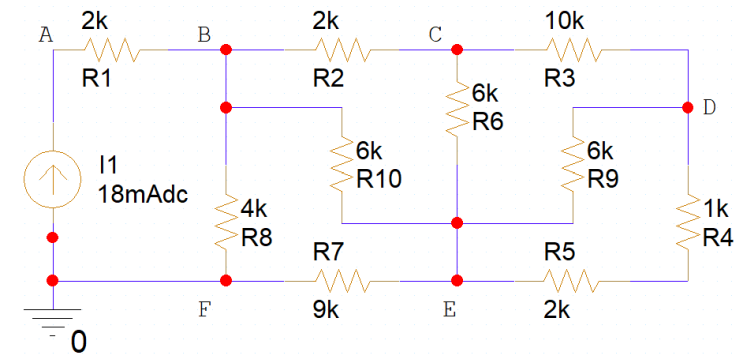
\includegraphics[width=0.7\textwidth]{graphics/ex3/f2.PNG}
\end{figure}